\chapter{Materials and methods}\label{chap:MatlsMethds}
A series of batch shaking tests were conducted to test the sorption strength of waste based biochars to PFAS and try to gain some insights into possible sorption mechanisms. The experiments were conducted using six perfluorinated carboxylic acids (C5-C10) to investigate how chain length affects sorption with and without the presence of soil, and both single compound and a cocktail of C5-C10 batch tests were performed to determine attenuation factors. A methods flowchart is given in \cref{fig:methodoverview}. The main work and laboratory experiments were conducted in the environmental chemistry laboratory at NGI, Oslo. The quantification analysis of the batch test filtrates was performed by UPLC-MS/MS at the Institute for Chemistry of Norwegian University of Science and Technology (NTNU), Trondheim. 

\begin{figure}
    \centering
    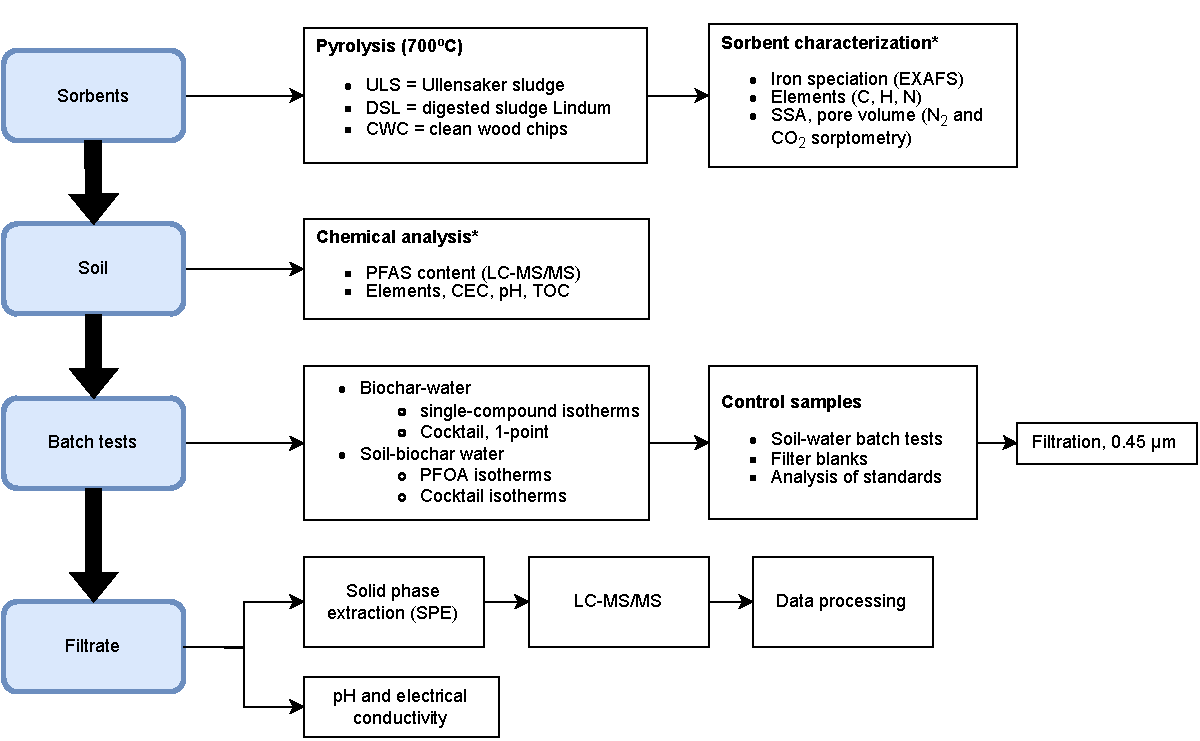
\includegraphics[width=\textwidth]{Diagrams/Methods-General_overview_methods.pdf}
    \caption{Overview of the methods conducted for this thesis. * = analyses conducted by commercial laboratories or that were delegated to project partners.}
    \label{fig:methodoverview}
\end{figure}

\section{Biochar sorbents}

\subsection{Feedstock}
Three feedstock types were selected as sorbents in the sorption experiments: Ullensaker Sludge (ULS), Digested Sludge Lindum (DSL) clean wood chips (CWC). ULS is raw sewage sludge from Ullensaker WWTP that has been dewatered. DSL is sewage sludge that has been through anaerobic digestion (AD) to produce biogas, also referred to as digestate. Anaerobic digestion is performed at Lindum AS and produces methane (and other gases; \cref{eq:AD}) which becomes commercial biogas fuel. The sewage sludge is dewatered, dried and pelletized before pyrolysis. CWC is made of clean, fresh softwood timber without additives that have been shredded, dried, and compressed into 8 mm pellets. The wood pellets are commercially available from Hallingdal trepellets (Kleivi næringspark, Ål).

\subsection{Pyrolysis}
CWC, ULS, and DSL biochars were produced by slow pyrolysis at 700 \textdegree C using ETIA technology by Biogreen\textsuperscript{\textcopyright} at Lindum AS (Drammen, Norway). \cref{tab:sorbents} summarizes the variables for pyrolysis of each biochar. The three biochars were produced as part of a larger study on the life cycle of waste based sorbents and was given as biochar samples to conduct the sorption experiments on for this thesis. The pyrolysis chamber is first electrically heated to stable PT. Feedstock pellets are added to a feeding container where a heated rotating screw (Spirajoule\textsuperscript{\textregistered}) transports the feedstock into and through the pyrolysis chamber at the programmed RT. The biochar is then transported to an external collection container where it is dispensed into sampling bags \cref{fig:biocharCollection}. \cref{fig:pellets} shows the pellets before and after pyrolysis. 

\begin{table}
\centering
\caption{Pyrolysis temperature (PT), residence time (RT) and feedstock for the biochars used in the sorption experiments.}
\label{tab:sorbents}
\begin{tabular}{llll}
\toprule
Biochar   & PT & RT & Feedstock \\
sorbent & (\textdegree C) & (min) \\
\midrule
CWC  & 700 & 20 & clean wood chips  \\
ULS & 700 & 40  & Ullensaker sludge\\
DSL & 700 & 20 & Digested sludge Lindum \\
\bottomrule
\end{tabular}
\end{table}

\begin{figure}
    \centering
    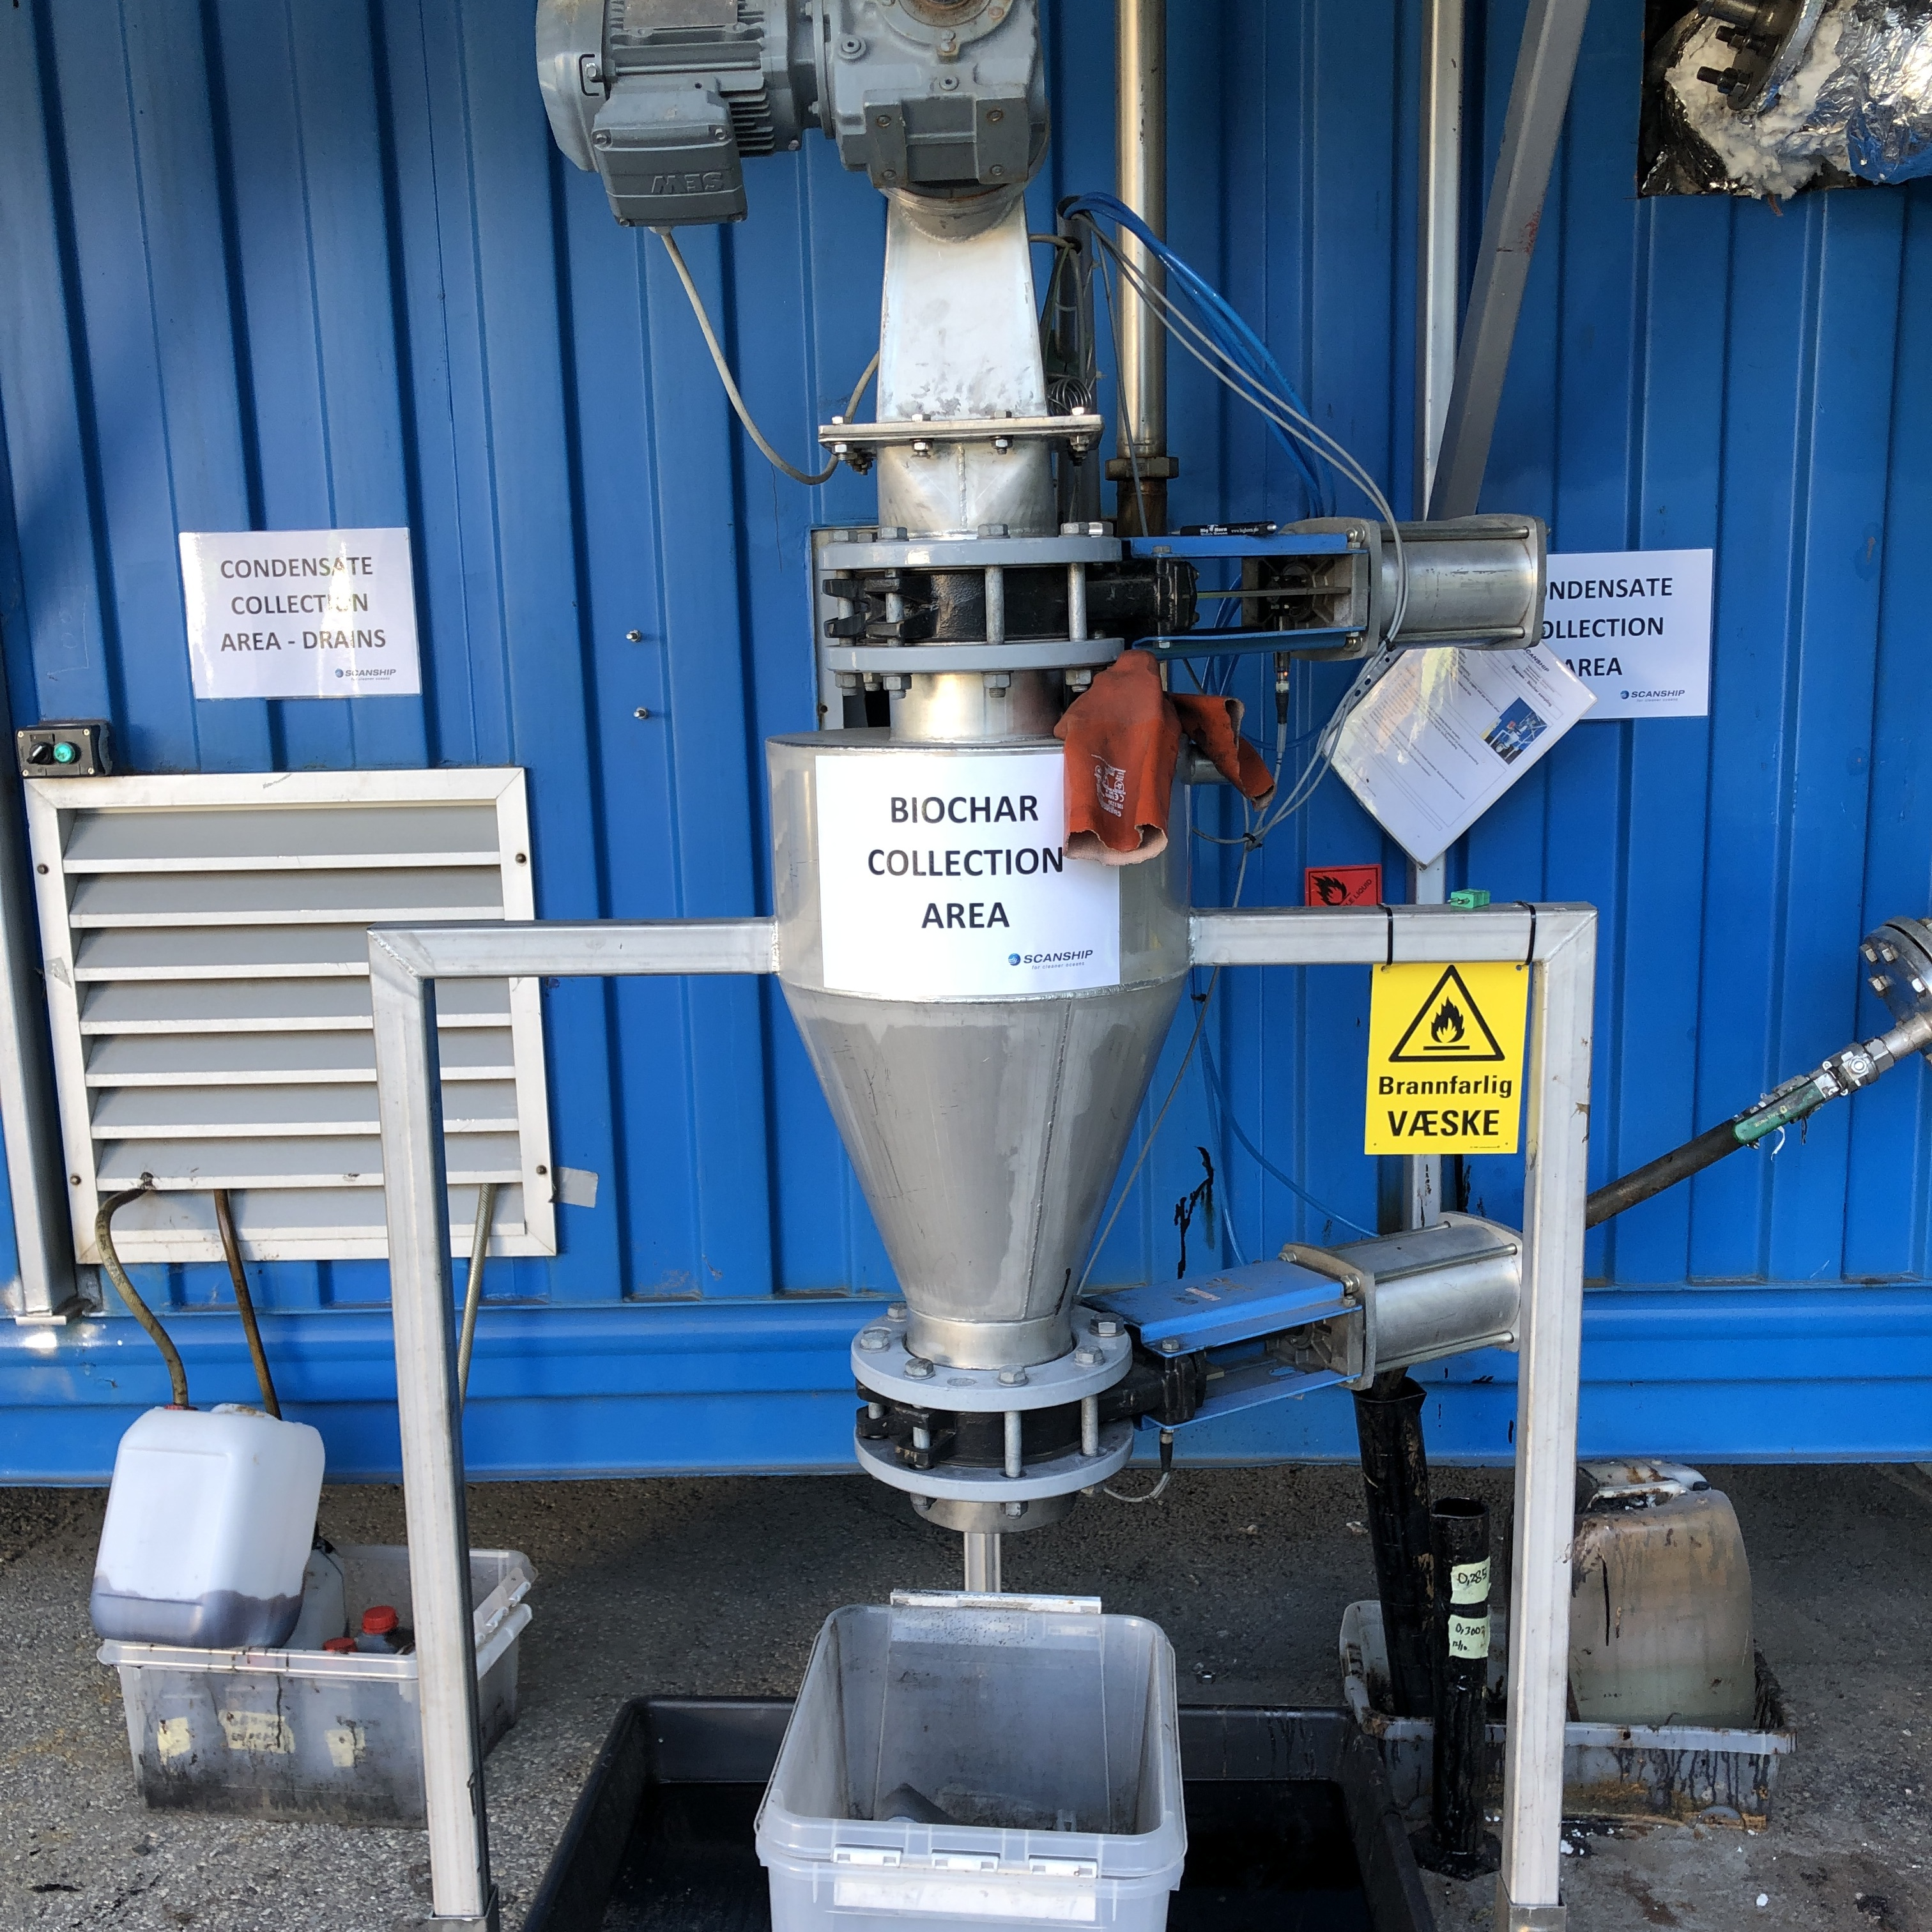
\includegraphics[width=0.6\linewidth,scale=0.6]{Bilder/Pyrolysis/BiocharCollection.jpg}
    \caption{Biochar collection area.}
    \label{fig:biocharCollection}
\end{figure}

\begin{figure}
    \centering
    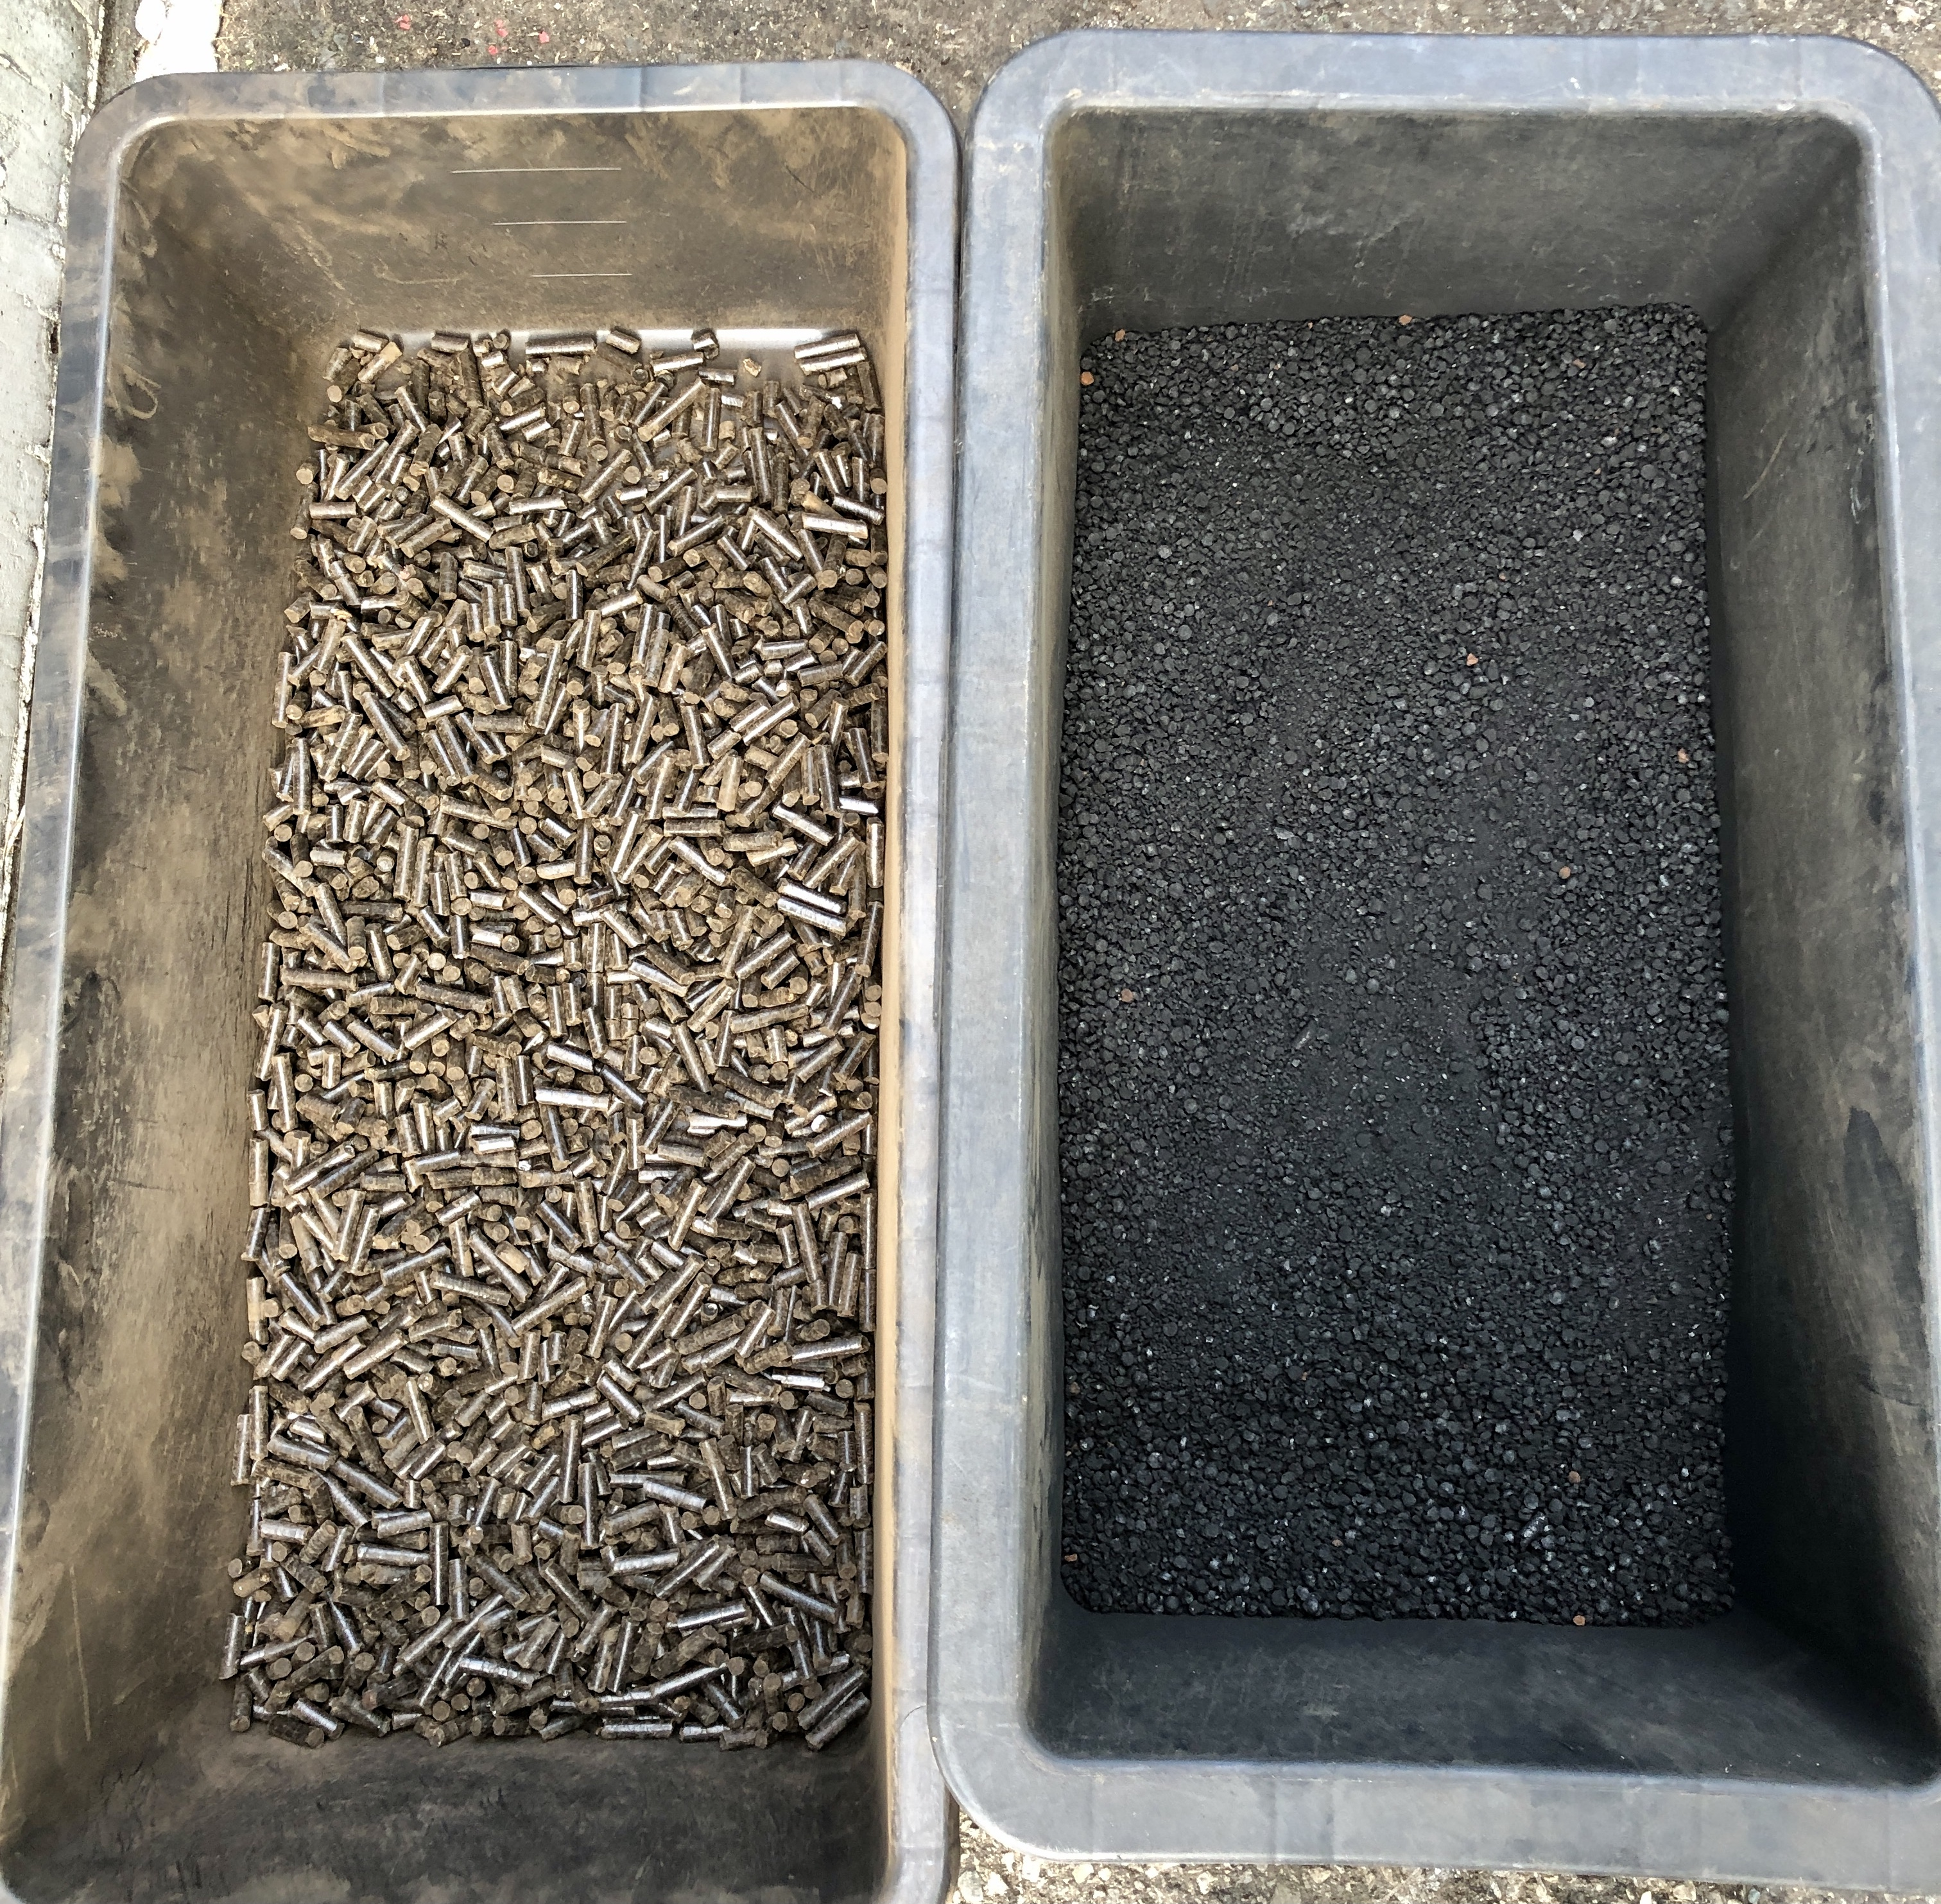
\includegraphics[width=0.6\linewidth,scale=0.6]{Bilder/Pyrolysis/Pellets.png}
    \caption{DSL feedstock pellets (left) and pyrolyzed pellets/biochar (right).}
    \label{fig:pellets}
\end{figure}

Syn-gas from pyrolysis is led through a condensing pipe that condenses into bio-oil at two points depending on boiling point. Syn-gas that does not condense at this point is led into a combustion chamber where a steady inflow of propane ensures a clean burning process of the remaining molecules. See \cref{appSec:pollution} for additional work on measurements on environmental pollutant emission from the ETIA unit.

\subsection{Biochar characterization}

\subsubsection{Surface area and pore volume}
Total specific surface area and pore volume were determined by $\mathrm{N_2}$ and $\mathrm{CO_2}$ gas sorptiometry by research partners at the Particle Engineering Research Center, University of Florida (Gainesville, USA) with a Quantachrome Autosorb 1 surface area analyzer according to the methods described by \cite{kwon2005}.  $\mathrm{N_2}$ sorptiometry was performed at the boiling point for liquid nitrogen (-195.8 \textdegree C). Due to slow diffusion at this low temperature, sorption of  $\mathrm{N_2}$ represents the largest pores of \textgreater 1.5 nm. $\mathrm{CO_2}$ sorptiometry was performed at 0 \textdegree C, and the higher temperature allows the gas to diffuse into smaller pores between 0.4-1.5 nm. $\mathrm{N_2}$ surface area was interpreted using Brunauer, Emmett and Teller (BET) theory, pore size and volume using Barret-Joyner-Halenda (BJH) theory, and $\mathrm{CO_2}$ surface area and pore volume were evaluated using density functional theory (DFT) theory . 

\subsubsection{Element analysis}
Elemental composition (total C, H and N) was performed by $\mathrm{NO_3}$ digestion and quantified with a Leco CHN-1000 from Leco Corporations (Sollentuna, Sweden), according to DIN 51732 by project partner.  

\subsubsection{Iron speciation}
Iron and copper speciation of DSL and ULS were analyzed by Fe K-edge X-ray absorption fine structures (EXAFS) at the synchrotron SOLEIL (Gif-sur-Yvette, France) (beamline SAMBA) by a project colleague at NGI. To prepare the biochars for analysis, each sample ($\sim$50 mg) was crushed with a mortar to a fine powder (250 \textmu m). The samples were mixed with boron nitride (BN, 300 mg) to a homogeneous powder and pelletized. BN matrix is used for sample dilution because it absorbs very little of the photon beam at the Fe K-edge. The biochar pellet was then analyzed by X-ray absorption spectroscopy.  

The overall principle of EXAFS is to determine structural composition of a sample by examining its X-ray absorption spectrum, which plots absorbance, $\mu x$, as a function of photon energy, $eV$ \citep{vlaica2004exafs}. The sample is submitted to an X-ray beam where a spectrophotometer measures the beam intensity going through the sample. The difference of intensity between before and after the sample is translated into an absorption coefficient, following Beer-Lambert's Law: 

\begin{equation}\label{eq:absorbance}
    \mu x = log \frac{I}{I_0}
\end{equation}

where $\mu x$ is a dimensionless absorbance coefficient ($AU$), $I$ is the transmitted light intensity and $I_0$ is the incident light intensity. The energy of the photon beam is determined by the angle of a crystal monochromator. The angle of the crystal monochromator is tuned so that the sample is submitted to a range of photon energies in which the absorption edges of the target element lie within \citep{vlaica2004exafs}. An adsorption K-edge occurs when the transmitted photon energy equals the energy required to excite a core electron, which is observed as a vertical jump (K) in $\mu x$ on the spectrum \citep{vlaica2004exafs}. The neighboring elements are interfering with the photon wave, which translates into oscillations on the absorption spectrum following the absorption edge. Each element has a different retrodiffusion coefficient, therefore the frequency and amplitude of oscillations in the absorption spectrum are (partially) determined by the type and number of neighboring atoms. The absorption edge energy and the oscillations thus contain information on the valency of the element and number and type of neighboring atoms, i.e., the element speciation. Fe(II) species will have K at a lower energy than Fe(III) species because a higher photon energy is required to excite an electron from the more electronegative Fe(III). In addition, the oscillations will differ depending on the Fe mineral. By interpreting the X-ray absorption spectrum, the different iron species present in the sample can be derived.

%%%%%%%%%%%%%%%%%%%%%%%%%%%%%%%%%%%%%%%%%%%%%%%%%%%%%%%%%%%%%%%%%%%%%%%%%%%%%%%%%%%%%%%%%%%%%%%%%%%%%%%%%%%%%%%

\section{Sorption experiments}
Effectiveness of PFCA removal by waste biochar was evaluated by batch shaking tests. The following section describes how the batch tests were prepared.

\subsection{Experiment preparations}
\subsubsection{Target compounds}\label{sec:PFCAanalytic}
Six perfluorinated carboxylic acids (PFCAs): perfluoropentanoic acid (PFPeA), perfluorohexanoic acid (PFHxA), perfluoroheptanoic acid (PFHpA), perfluorooctanoic acid (PFOA), perfluorononaoic acid (PFNA), perfluorodecanoic acid (PFDA), with perfluorinated carbon (PFC) units 4-9 respectively were chosen as sorbates for the batch test experiments in this thesis. Hereafter, these are referred to as target compounds/TCs. See \cref{tab:PFCAs} for a list of all native PFCAs including their respective CAS numbers included in this thesis. 10 mL stock solutions were prepared for each TC by weighing the pure PFCA salts/liquid (\cref{tab:PFCAs}) on an analytical scale and dissolving them in methanol in volumetric flasks. Two spiking standards at a high (STD1) and low (STD2) concentration were prepared from the stock solution to be used for spiking the batch tests at various concentrations (\cref{apptab:standards}). The working standards were analyzed with LC-MS/MS of a 2-time diluted standard at an optimum concentration for the instrument calibration curve (10-20 \textmu g L\textsuperscript{-1}, \cref{appSec:IsothermSetup}) and all further calculations of spike dilutions were corrected with the measured standard concentrations.

\begin{table}
\centering
\caption{PFAS compounds investigated in this study. PFCs correspond to the number of perfluorinated carbon units in the chain. Note: PFCAs appear in dissociated form at environmentally relevant pH's due to low $pK_a$'s.}
\adjustbox{max width=\textwidth}{
\label{tab:PFCAs}
\begin{tabular}{@{}lcccclc@{}}
\toprule
\multicolumn{1}{c}{Chemical} & Acronym & Short & CAS number & Molecular structure & Stock form & Purity \\ \midrule
& & & & & &\\
\smash{\raisebox{4ex}{Perfluoropentanoic acid}}  & \smash{\raisebox{4ex}{PFPeA}} & \smash{\raisebox{4ex}{C5}} & \smash{\raisebox{4ex}{2706-90-3}} & \chemfig[atom style={scale=0.4}]{O=[:90](-[:30,,,1]OH)-[:150](-[:112.5]F)(-[:67.5]F)-[:210](-[:292.5]F)(-[:247.5]F)-[:150](-[:112.5]F)(-[:67.5]F)-[:210](-[:270]F)(-[:150]F)-[:210]F} & \smash{\raisebox{4ex}{liquid}} & \smash{\raisebox{4ex}{\textgreater 97 \%}} \\
& & & & & &\\
\smash{\raisebox{4ex}{Perfluorohexanoic acid}} & \smash{\raisebox{4ex}{PFHxA}}  & \smash{\raisebox{4ex}{C6}} & \smash{\raisebox{4ex}{307-24-4}} & \chemfig[atom style={scale=0.4}]{O=[:90](-[:30,,,1]OH)-[:150](-[:112.5]F)(-[:67.5]F)-[:210](-[:292.5]F)(-[:247.5]F)-[:150](-[:112.5]F)(-[:67.5]F)-[:210](-[:292.5]F)(-[:247.5]F)-[:150](-[:210]F)(-[:150]F)-[:90]F} & \smash{\raisebox{4ex}{liquid}} & \smash{\raisebox{4ex}{\textgreater 97 \%}} \\
& & & & & &\\
\smash{\raisebox{4ex}{Perfluoroheptanoic acid}} & \smash{\raisebox{4ex}{PFHpA}} & \smash{\raisebox{4ex}{C7}} & \smash{\raisebox{4ex}{375-85-9}} & \chemfig[atom style={scale=0.4}]{O=[:90](-[:30,,,1]OH)-[:150](-[:67.5]F)(-[:112.5]F)-[:210](-[:247.5]F)(-[:292.5]F)-[:150](-[:67.5]F)(-[:112.5]F)-[:210](-[:247.5]F)(-[:292.5]F)-[:150](-[:67.5]F)(-[:112.5]F)-[:210](-[:150]F)(-[:210]F)-[:270]F} & \smash{\raisebox{4ex}{crystalline}} & \smash{\raisebox{4ex}{\textgreater 99 \%}} \\
& & & & & &\\
\smash{\raisebox{4ex}{Perfluorooctanoic acid}} & \smash{\raisebox{4ex}{PFOA}}  & \smash{\raisebox{4ex}{C8}} & \smash{\raisebox{4ex}{335-76-2}}  & \chemfig[atom style={scale=0.4}]{O=[:90](-[:30,,,1]OH)-[:150](-[:67.5]F)(-[:112.5]F)-[:210](-[:247.5]F)(-[:292.5]F)-[:150](-[:67.5]F)(-[:112.5]F)-[:210](-[:247.5]F)(-[:292.5]F)-[:150](-[:67.5]F)(-[:112.5]F)-[:210](-[:247.5]F)(-[:292.5]F)-[:150](-[:90]F)(-[:150]F)-[:210]F} & \smash{\raisebox{4ex}{powder}} & \smash{\raisebox{4ex}{\textgreater 95 \%}} \\
& & & & & &\\
\smash{\raisebox{4ex}{Perfluorononaoic acid}}  & \smash{\raisebox{4ex}{PFNA}} & \smash{\raisebox{4ex}{C9}} & \smash{\raisebox{4ex}{375-95-1}} & \chemfig[atom style={scale=0.4}]{O=[:90](-[:30,,,1]OH)-[:150](-[:112.5]F)(-[:67.5]F)-[:210](-[:292.5]F)(-[:247.5]F)-[:150](-[:112.5]F)(-[:67.5]F)-[:210](-[:292.5])(-[:247.5]F)-[:150](-[:112.5]F)(-[:67.5]F)-[:210](-[:292.5]F)(-[:247.5]F)-[:150](-[:112.5]F)(-[:67.5]F)-[:210](-[:270]F)(-[:210]F)-[:150]F} & \smash{\raisebox{4ex}{crystalline}} & \smash{\raisebox{4ex}{\textgreater 97 \%}} \\
& & & & & &\\
\smash{\raisebox{4ex}{Perfluorodecanoic acid}}  & \smash{\raisebox{4ex}{PFDA}}  & \smash{\raisebox{4ex}{C10}} & \smash{\raisebox{4ex}{335-67-1}} & \chemfig[atom style={scale=0.4}]{O=[:90](-[:30,,,1]OH)-[:150](-[:112.5]F)(-[:67.5]F)-[:210](-[:292.5]F)(-[:247.5]F)-[:150](-[:112.5]F)(-[:67.5]F)-[:210](-[:292.5]F)(-[:247.5]F)-[:150](-[:112.5]F)(-[:67.5]F)-[:210](-[:292.5]F)(-[:247.5]F)-[:150](-[:112.5]F)(-[:67.5]F)-[:210](-[:292.5]F)(-[:247.5]F)-[:150](-[:210]F)(-[:150]F)-[:90]F} & \smash{\raisebox{4ex}{flakes}} & \smash{\raisebox{4ex}{\textgreater 98\%}} \\
& & & & & &\\ \bottomrule
\end{tabular}}
\end{table}

\subsubsection{Spike concentrations}
Sorption of PFAS to biochar follows the Freundlich sorption model, which means that sorption increases linearly until it is attenuated at higher concentrations \cref{eq:Freundlich}. The goal when designing the sorption isotherm experiments was to represent sorption across both the linear and non-linear region. To achieve detectable concentrations across this range, determination of appropriate spike concentrations was based on several factors: 1) Biochar-water partition coefficients ($K_{BC}$) for the TCs obtained from literature \cite{Xiao2017} \cref{tab:Kbc}, 2) biochar dose, 3), the LOQ of the analytical method, and 4) available pipetting volume range. The relationship between $K_{BC}~\mathrm{(L~g^{-1})}$, the sorbed concentration, $C_s~\mathrm{(\mu g~g^{-1})}$, and the freely dissolved aqueous concentration, $C_w~\mathrm{(\mu g~L^{-1})}$, expressed as:

\begin{align}
    \label{eq:Kbc1}
    K_{d} = \frac{C_s}{C_w}
\end{align}

was used to estimate the expected $C_w$. By rearranging \cref{eq:Kbc1},  $C_w$ is expressed as a function of the mass TA spiked and the estimated $K_d$:

\begin{align}
    \label{eq:Cw2}
    C_w=\frac{\frac{m_{PFAS}}{\left (\frac{m_{BC}\times K_{BC}}{V_w}\right)+1}}{V_w}
\end{align}

Where $m_{TA}$ is the mass PFAS spiked, $m_{BC}$ is the biochar dose, and $V_w$ is the volume of the sample matrix. Using \cref{eq:Cw2}, the lowest spike concentration for each isotherm was taken to be two times the method LOQ for the LC-MS/MS instrument at NTNU, Trondheim (\cref{apptab:LOQ}). The remaining points were spread evenly over a $10^4$ concentration interval. 

\begin{table}
\centering
\caption{Biochar-water distribution coefficients ($K_{BC}$) for PFCAs derived from \cite{XiaoSI2017}.} 
\label{tab:Kbc}
\begin{threeparttable}
    \begin{tabular}{@{}lcc@{}}
    \toprule
    \multicolumn{1}{l}{\begin{tabular}[l]{@{}l@{}}Compound\end{tabular}} &  \multicolumn{1}{c}{\begin{tabular}[c]{@{}c@{}}log $\mathrm{K_{BC}}$\\ \citep{XiaoSI2017}\end{tabular}} & \multicolumn{1}{c}{\begin{tabular}[c]{@{}c@{}}est. log $\mathrm{K_{BC}}$ \end{tabular}} \\ \midrule
    PFPeA & 4.16 & 4.16 \\
    PFHxA & 4.15 & 4.15 \\
    PFHpA & 4.49 & 4.49 \\
    PFOA & 4.76 & 4.76 \\
    PFNA & *4.89 & 4.89 \\
    PFDA & *5.09 & 5.09 \\ \bottomrule             
    \end{tabular}
\begin{tablenotes}
\item * not included in \citep{XiaoSI2017}, so the values are extrapolated from the shorter chain lengths.
\end{tablenotes}
\end{threeparttable}
\end{table}

Two preliminary batch tests were prepared to check how well the $K_d$ values selected from the literature corresponded to those for ULS and CWC. Further details about this analysis are provided in \cref{appSec:IsothermSetup}.

\subsubsection{Biochar}
A sub sample (100 g) was taken by random grab sampling from the bulk volume of the biochar produced during the pyrolysis run. The biochars were crushed using a ball mill (Retsch ISO 9001) with five balls at 50 rpm for 5 minutes and sieved into fine-powdered biochar (D \textless 1 mm) and transferred to LDPE zipper bags for storage (4 \textdegree C). 

\subsubsection{Soil}
The soil used for the sorption tests was an unaged sandy soil obtained from a remote field area 17 km from Uppsala, Sweden (59.733 N, 17.667 E). TOC-content was determined according to... pH according to... The soil was characterized for total element concentrations, exchangeable ions, TOC and pH by... the methods... The soil was dried at 100 \textdegree C for 24 h and crushed and sieved to \textless 2 mm.  The soil was screened for PFAS using a methanol extraction, solid phase extraction and quantification by liquid chromatography coupled with tandem mass spectrometry at NTNU (Trondheim, Norway) by a project partner (details for the SPE and LC-MS/MS procedures will be given in \cref{methods:instrAnalysis}), performed in triplicate.

\begin{figure}
    \centering
    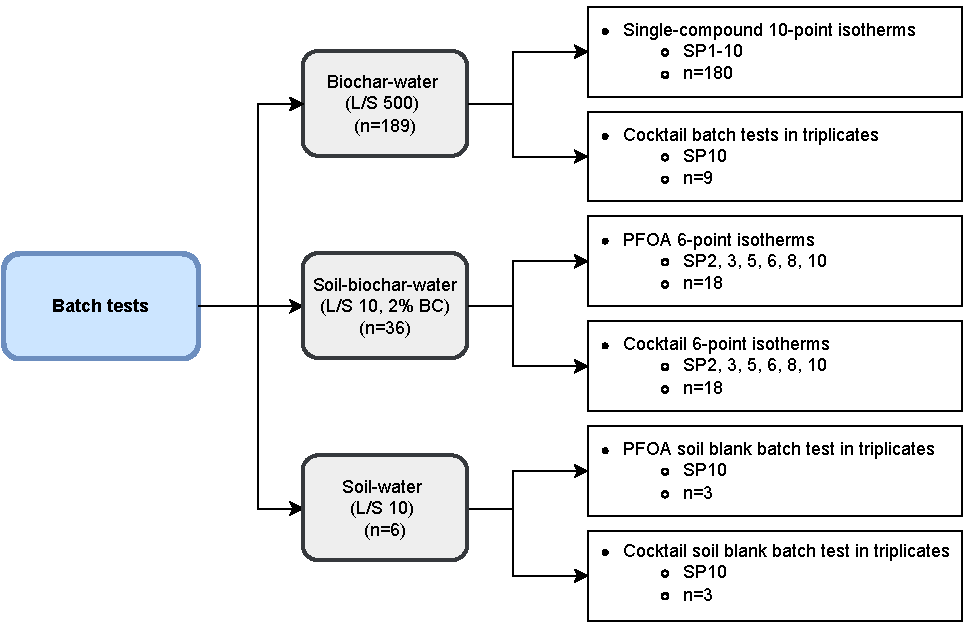
\includegraphics{Diagrams/Methods-Page-9.pdf}
    \caption{Overview of batch test samples for this thesis for the three biochars (ULS, DSL, CWC) and six TCs.}
    \label{fig:batchtests}
\end{figure}

\begin{table}
    \caption{Spike concentrations (SC) in \textmu g L\textsuperscript{-1} used for the batch tests. MIX = cocktail spike concentration for biochar-water batch tests in triplicates, MIX-S = cocktail spike concentration for biochar-soil-water and soil-water batch tests.}
    \label{tab:spikeConcentrations}
    \adjustbox{max width=\textwidth}{%
    \begin{tabular}{lrrrrrrrrrrrr}
    \toprule
    \textbf{Compound} & \textbf{SC1} & \textbf{SC2} & \textbf{SC3} & \textbf{SC4} & \textbf{SC5} & \textbf{SC6} & \textbf{SC7} & \textbf{SC8} & \textbf{SC9} & \textbf{SC10} & \textbf{SC10-MIX} & \textbf{SC10-MIX-S} \\ \midrule
    PFPeA & 0.019 & 21 & 43 & 64 & 86 & 107 & 128 & 150 & 171 & 191 & 191 & 283\\
    PFHxA & 0.033 & 37 & 73 & 110 & 146 & 184 & 220 & 256 & 292 & 330 & 330 & 836 \\
    PFHpA & 0.012 & 11 & 25 & 38 & 52 & 65 & 79 & 92 & 106 & 117 & 117 & 153\\
    PFOA & 0.195 & 216 & 435 & 651 & 871 & 1 087 & 1 302 & 1 522 & 1 742 & 1 953 & 1 953 & 1 974\\
    PFNA & 0.141 & 156 & 313 & 471 & 625 & 784 & 942 & 1 097 & 1 255 & 1 409 & 1 409 & 2 310\\
    PFDA & 0.383 & 425 & 850 & 1 275 & 1 700 & 2 126 & 2 551 & 2 976 & 3 401 & 3 830 & 3 830 & 5 288\\ \bottomrule
    \end{tabular}}
\end{table}

\subsection{Batch tests}
An overview of the experimental setup for the batch test is given in \cref{fig:batchtests}. Details for the preparations of each batch test category are given in the subsections below. The batch tests were prepared with a liquid to solid mass ratio (L/S) of 500 for biochar and L/S of 10 for soil amended with 2\% biochar in accordance with CEN EN 12457. The dry matter was added to pre-cleaned 50 mL PP centrifuge tubes and spiked with either individual PFCAs or a cocktail of all six TCs at the concentrations specified in \cref{tab:spikeConcentrations} to a final liquid volume of 50 mL. The standard concentrations were analytically verified to ensure accuracy of the data analysis (see \cref{appSec:IsothermSetup} for expected vs. analytical concentrations). The samples were assured to contain \textless 10\% MeOH, which is the upper limit for which methanol does not influence sorption (reference). The batch tests were shaken end-over-end (9 rpm) and/or agitated on a shaking table (160 rpm) in room temperature (20\textdegree C) for at least 14 days to reach equilibrium \citep{higgins2006sorption} before filtration through a 0.45 \textmu m Minisart\textsuperscript{\textregistered} regenerated cellulose syringe filter into PP tubes based on the methods described in \cite{Sorengard2019}. Loss of biochar to the walls of the syringe was quantified to maintain a full mass balance when analyzing the partitioning of the TCs between the solid and liquid phase and is in \cref{appSec:misclab}. Therefore, a 100\% mass balance was assumed when calculating partitioning between sorbent and water by subtracting the initial spike concentration from the measured concentration in the filtrates. by also correcting for loss to laboratory ware (reference). 

\subsubsection{Biochar-water batch tests}
100\textpm 4 mg biochar was weighed for the biochar-water batch tests. on an analytical scale and placed into pre-cleaned (50\% methanol) 50 mL PP tubes. The tubes were filled half up of Milli-Q water. In each tube, stock PFCA was pipetted using micro- (5-50 {\textmu}l and 200-1000 {\textmu}L) and milli pipettes (2-10 mL) into the char-water solution to make 10 dilutions for each of the 6 PFCAs in even intervals within the concentration points in \cref{tab:spikeConcentrations}. Some tubes were added Milli-Q water up to the 50 mL mark and some were weighed in order to control for the water amount being within \textpm 0.02 mL. The same ten concentrations were used to spike CWC, ULS and DSL batch tests. A cocktail batch test was prepared for the three biochars at SP10  The same dose biochar was used as for the other sorption isotherms. The cumulative CMC (critical micelle concentration) for the six PFCAs at SC10 was assured not to be an issue for the concentration range considered \citep{bhhatarai2011,ding2013physicochemical}.

\subsubsection{Soil-biochar-water batch tests}
5\textpm 0.005 g soil, 0.1\textpm 0.0004 g biochar
The batch tests were prepared as 6-point isotherms within a 10\textsuperscript{4} concentration range with a L/S ratio of 10 in PP tubes, in accordance with CEN EN 12457 with modifications described in \citep{Hale2017fire,Kupryianchyk2016a}. L/S 10  is common in leaching tests for waste materials and soil according to the waste and shaken in an end-over-end shaker for \textgreater 14 days. 
centrifuged to remove as many particles from suspension as possible. Still, filtration required frequent filter change due to clogging (up to three times per sample).

\subsection{pH and electrical conductivity}
pH and conductivity was measured in a solution (1:5) of biochar and water, with pre-stirring (15 min) and letting the particles settle (\textgreater 24 hrs) before measurement (n=3). This is according to the standard method for measuring pH in soil. It is common to add CaCl\textsubscript{2} if the soil has a low ionic strength, but this was considered unnecessary in the presence of biochar as it contains a high amount of soluble ions. 

\subsection{Control samples}
To prevent underestimation of $C_w$, filter blanks were prepared for each PFCA in triplicates at an optimum concentration range for the instrument (see \cref{sec:PFCAanalytic}) to correct for PFCA loss to the filter paper. 

%%%%%%%%%%%%%%%%%%%%%%%%%%%%%%%%%%%%%%%%%%%%%%%%%%%%%%%%%%%%%%%%%%%%%%%%%%%%%%%%%%%%%%%%%%%%%%%%%%%%%%%%%%%%%%%%%%%%%%%%%%%%

\section{Instrumental analysis} \label{methods:instrAnalysis}
PFAS quantitation in the filtrates were determined by liquid chromatography--tandem mass spectrometry (LC-MS/MS). Reversed phase solid phase extraction (SPE) was used as sample preparation method. The analyses were conducted at the Institute of Chemistry at NTNU (Trondheim, Norway).

% missing reconstitution step, update diagram
\begin{figure}
    \centering
    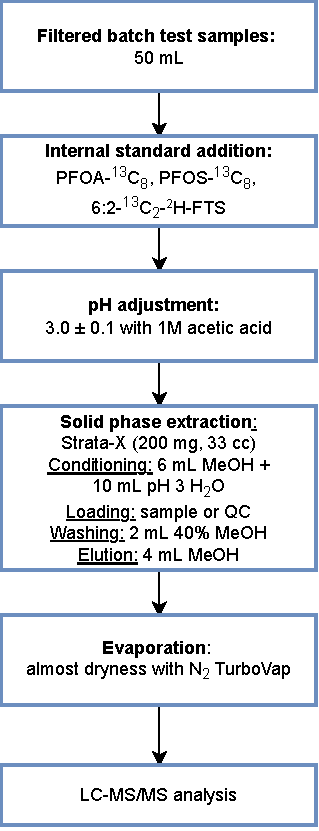
\includegraphics{Diagrams/Methods-Analytical_method.pdf}
    \caption{Schematic diagram of the analytical method applied for the determination of TCs in the batch test filtrates adapted from \cite{arvaniti2012diagram}.}
    \label{fig:analyticalMethod}
\end{figure}

\subsection{SPE}
SPE is a sample preparation method used to concentrate a large-volume sample to an extract that can be submitted for analyte quantitation by LC-MS/MS. The sample is passed through a cartridge with a porous sorbent polymer that strongly retains polar compounds (\textpi-\textpi bonding, hydrogen bonding and hydrophobic interaction). The sorbed analytes are then eluted with an appropriate solvent, evaporated, and finally reconstituted to the desired extract volume. All samples are spiked with a mix of internal standards (ISs) to compensate for variations in extraction percentages and instrumental response by the MS/MS detector \citep{arvaniti2014}. To minimize risk of contamination during laboratory work, working benches were cleaned with acetone and covered with aluminum foil. Sterilized PP tubes were used during all steps of the protocol.

Strata-X\textsuperscript{\textregistered} 200 mg/6mL cartridges supplied by Phenomenex were used for SPE of the TCs in the filtered water samples. The sorbent polymer was a surface modified styrene divinylbenzene (\cref{fig:StatPhase}) with 33 \textmu m average particle diameter and surface area of 800 m\textsuperscript{2} g\textsuperscript{-1}. The internal standards used were \textsuperscript{13}C\textsubscript{8}-perfluorooctanoic acid  (\textsuperscript{13}C\textsubscript{8}-PFOA), \textsuperscript{13}C\textsubscript{8}-potassium perfluorooctanesulfonate (\textsuperscript{13}C\textsubscript{8}-PFOS-K), and 6:2-\textsuperscript{13}C\textsubscript{2}-\textsuperscript{1}H,\textsuperscript{2}H-perfluorooctane sulfonate  (6:2 \textsuperscript{13}C\textsubscript{2}-FTS) where a working standard of the three isotopic PFAS was prepared in methanol at 1 ppm from 50 ppm analytical standard supplied by Sigma Aldrich.

The samples were adjusted to pH $\sim$3 with 800 \textmu L 1 M acetic acid. However, the samples containing soil needed addition of at least double the amount to reach the same pH. pH was tested for five randomly selected samples for each batch of 20 was with pH strips. All samples were then spiked with IS. SC1 and SC2 samples were spiked with 10 \textmu L IS and SC3-SC10 samples were spiked with 20 \textmu L IS--the difference in amount of IS for the two low-spike samples being due to a more concentrated extract needed for these samples to avoid signals below instrumental LOQ. Therefore, SC1 and SC2 samples were made to 0.5 mL extracts instead of 1 mL as for the rest. The samples were vortexed prior to SPE.

The cartridges were placed in individual slots with LC liners on a TLC chamber and conditioned with 6 mL MeOH and 10 mL pH 3 milli-Q water (acidified by 100\% acetic acid). MeOH was used for wetting to allow the mobile phase into the pores of the sorbent polymer in order to ensure maximum chromatographic retention. Low-pH water was used to protonate loan electrons on the polymer surface so that hydrophobic interaction with the analytes were maximized. The samples were loaded using glass pipettes and allowed to pass through the cartridges with gravity. The flow rate was adjusted by modifying the opening of the LC liners so that the sample exited the cartridge as individual droplets. 

After loading the samples, the cartridges were washed with 2 mL MeOH:MQ (40:60, \% v/v) in order to remove any matrix interferences. The cartridges were then dried with a vacuum pump at 20 mmHg until the sorbent mass was visible as dry powder. The analytes were eluted with 4 mL MeOH into 15 mL PP centrifuge tubes, and concentrated to almost dryness ($\le$0.5 mL) using TurboVap\textsuperscript{\textregistered} at 40 \textdegree C and nitrogen gas (N\textsubscript{2}) at 5 psi. The samples were reconstituted to 1 mL (0.5 mL for SCs 1 and 2) with MeOH and milli Q to a final solvent ratio of 50:50 \% v/v. The extracts were transferred to LC vials using glass pipettes and stored at -19 \textdegree C until analysis.

\begin{figure}
    \centering
    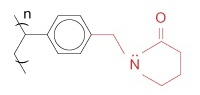
\includegraphics{Bilder/SPE_LCMS/mg_spe_strata-x.jpg}
    \caption{Sorbent polymer used for SPE, surface-modified styrene divinylbenzene.}
    \label{fig:StatPhase}
\end{figure}

\subsection{LC-MS/MS}
Liquid chromatography separates compounds in a mixture based on polarity by using a stationary phase that retards hydrophobic compounds while allowing more polar compounds to pass through faster along with the polar mobile phase. The compounds are then ionized by a strong voltage into fragment ions that are detected by a mass spectrometer that determines the mass of the transitions. Quantification of PFAS was determined by UPLC-MS/MS with an Acquity UPLC I-Class system connected to a Xevo TQ-S triple quadrupole mass spectrometer equipped with an ESI Z spray, both supplied by Waters (Milford, MA, USA). A Kinetex C18 column (30 x 2.1 mm, 1.3 \textmu m) serially connected to a Phenomenex C18 (2 x 2.1 mm i.d.) security guard (Torrance, CA, USA) was used for chromatographic separation. Mobile phases were A: 2 mM ammonium acetate in Milli-Q water (water phase) and B: pure MeOH (organic phase) that were supplied at a constant flow rate of 250 \textmu L min\textsuperscript{-1} to the LC column maintained at a temperature of 30 \textdegree C. The sample injection volume was 4 \textmu L. The run time for each sample was 6 minutes with an initial and final mobile phase gradient of 20:80 (A:B). Analytes were ionized by negative electrospray ionization (ESI-) and nitrogen was used as drying gas at the ionization source. Two ion transitions were monitored for each PFCA (\cref{tab:transitions}) within 60 s of the expected retention time for the compound. Peak integration was performed automatically by MassLynx software obtaining 12 points per peak and an average baseline peak width of 5 s. Data from UPLC-MS/MS was processed in MassLynx version 4.1 and quantification processing was performed with TargetLynx. Each peak was manually reviewed to remove peaks that were likely background noise as well as corrections for inconsistencies in peak base width. Complete instrument programming and parameters are summarized in \cref{appSec:LCMS}.

\begin{table}[tbh]
\centering
\caption{Ion transitions for the target analytes and internal standards in this study.}
\adjustbox{max width=\textwidth}{%
\begin{threeparttable}
\label{tab:transitions}
\begin{tabular}{ccccccl} \toprule
Compound &  Structure & Formula & M & Parent & Cone (V) & Transitions (CE)  \\ \midrule
& & & & & & \\
\multirow{2}{*}{PFPeA} &  \multirow{2}{*}{\chemfig[atom style={scale=0.5}]{O=[:90](-[:30,,,1]OH)-[:150](-[:112.5]F)(-[:67.5]F)-[:210](-[:292.5]F)(-[:247.5]F)-[:150](-[:112.5]F)(-[:67.5]F)-[:210](-[:270]F)(-[:150]F)-[:210]F}} & \multirow{2}{*}{$\mathrm{C_5HF_9O_2}$} & \multirow{2}{*}{264.05} & \multirow{2}{*}{262.97} & \multirow{2}{*}{20} & \multirow{2}{*}{262.97 $\rightarrow$ 219 (8)} \\
& & & & & & \\
& & & & & & \\
 &  &  &  &  &  &    \\
\multirow{2}{*}{PFHxA} &  \multirow{2}{*}{\chemfig[atom style={scale=0.5}]{O=[:90](-[:30,,,1]OH)-[:150](-[:112.5]F)(-[:67.5]F)-[:210](-[:292.5]F)(-[:247.5]F)-[:150](-[:112.5]F)(-[:67.5]F)-[:210](-[:292.5]F)(-[:247.5]F)-[:150](-[:210]F)(-[:150]F)-[:90]F}} & \multirow{2}{*}{$\mathrm{C_6HF_{11}O_2}$} & \multirow{2}{*}{314.05} & \multirow{2}{*}{312.97} & \multirow{2}{*}{10} & 312.97 $\rightarrow$ 118.95 (18) \\
 &  &  &  &  &  &   312.97 $\rightarrow$ 269 (8) \\
 & & & & & & \\
 & & & & & & \\
\multirow{2}{*}{PFHpA} &  \multirow{2}{*}{\chemfig[atom style={scale=0.5}]{O=[:90](-[:30,,,1]OH)-[:150](-[:67.5]F)(-[:112.5]F)-[:210](-[:247.5]F)(-[:292.5]F)-[:150](-[:67.5]F)(-[:112.5]F)-[:210](-[:247.5]F)(-[:292.5]F)-[:150](-[:67.5]F)(-[:112.5]F)-[:210](-[:150]F)(-[:210]F)-[:270]F}} & \multirow{2}{*}{$\mathrm{C_7HF_{13}O_2}$} & \multirow{2}{*}{364} & \multirow{2}{*}{362.96} & \multirow{2}{*}{6} & 362.96 $\rightarrow$ 119.00 (22) \\
 &  &  &  &  &  &   362.96 $\rightarrow$ 168.97 (18) \\
 & & & & & & \\
 & & & & & & \\
\multirow{2}{*}{PFOA} &  \multirow{2}{*}{\chemfig[atom style={scale=0.5}]{O=[:90](-[:30,,,1]OH)-[:150](-[:67.5]F)(-[:112.5]F)-[:210](-[:247.5]F)(-[:292.5]F)-[:150](-[:67.5]F)(-[:112.5]F)-[:210](-[:247.5]F)(-[:292.5]F)-[:150](-[:67.5]F)(-[:112.5]F)-[:210](-[:247.5]F)(-[:292.5]F)-[:150](-[:90]F)(-[:150]F)-[:210]F}} & \multirow{2}{*}{$\mathrm{C_8HF_{15}O_2}$} & \multirow{2}{*}{414.07} & \multirow{2}{*}{412.97} & \multirow{2}{*}{20} & 412.97 $\rightarrow$ 168.90 (18) \\
 &  &  &  &  &    & 412.97 $\rightarrow$ 369.00 (8) \\
 & & & & & & \\
 & & & & & & \\
\multirow{2}{*}{PFNA} &  \multirow{2}{*}{\chemfig[atom style={scale=0.5}]{O=[:90](-[:30,,,1]OH)-[:150](-[:112.5]F)(-[:67.5]F)-[:210](-[:292.5]F)(-[:247.5]F)-[:150](-[:112.5]F)(-[:67.5]F)-[:210](-[:292.5])(-[:247.5]F)-[:150](-[:112.5]F)(-[:67.5]F)-[:210](-[:292.5]F)(-[:247.5]F)-[:150](-[:112.5]F)(-[:67.5]F)-[:210](-[:270]F)(-[:210]F)-[:150]F}} & \multirow{2}{*}{$\mathrm{C_9HF_{17}O_2}$} & \multirow{2}{*}{464.08} & \multirow{2}{*}{462.99} & \multirow{2}{*}{20} & 462.99 $\rightarrow$ 219 (16) \\
 &  &  &  &  &    & 462.99 $\rightarrow$ 419 (10) \\
  & & & & & & \\
  & & & & & & \\
\multirow{2}{*}{PFDA} &  \multirow{2}{*}{\chemfig[atom style={scale=0.5}]{O=[:90](-[:30,,,1]OH)-[:150](-[:112.5]F)(-[:67.5]F)-[:210](-[:292.5]F)(-[:247.5]F)-[:150](-[:112.5]F)(-[:67.5]F)-[:210](-[:292.5]F)(-[:247.5]F)-[:150](-[:112.5]F)(-[:67.5]F)-[:210](-[:292.5]F)(-[:247.5]F)-[:150](-[:112.5]F)(-[:67.5]F)-[:210](-[:292.5]F)(-[:247.5]F)-[:150](-[:210]F)(-[:150]F)-[:90]F}} & \multirow{2}{*}{$\mathrm{C_{10}HF_{19}O_2}$} & \multirow{2}{*}{514.09} & \multirow{2}{*}{513.1} & \multirow{2}{*}{10} & 513.10 $\rightarrow$ 219.01 (18) \\
 &  &  &  &  &    & 513.10 $\rightarrow$ 269.04 (16) \\ 
 & & & & & & \\
 & & & & & & \\ \midrule
 \multicolumn{7}{c}{\textit{Internal standards (IS)}} \\ \midrule
  & & & & & & \\
 \multirow{2}{*}{PFOA \textsuperscript{13}C\textsubscript{8}} & \multirow{2}{*}{\chemfig[atom style={scale=0.5}]{O=[:90](-[:30,,,1]OH)-[:150](-[:67.5]F)(-[:112.5]F)-[:210](-[:247.5]F)(-[:292.5]F)-[:150](-[:67.5]F)(-[:112.5]F)-[:210](-[:247.5]F)(-[:292.5]F)-[:150](-[:67.5]F)(-[:112.5]F)-[:210](-[:247.5]F)(-[:292.5]F)-[:150](-[:90]F)(-[:150]F)-[:210]F}} & \multirow{2}{*}{$\mathrm{^{13}C_8HF_{15}O_2}$} & \multirow{2}{*}{422.01} & \multirow{2}{*}{420.9} & \multirow{2}{*}{16} & 420.90 $\rightarrow$ 171.86 (16) \\
 &  &  &  &  &    & 420.90 $\rightarrow$ 222.84 (16) \\ 
 & & & & & & \\
 & & & & & & \\
  \multirow{2}{*}{PFOS \textsuperscript{13}C\textsubscript{8}} & \multirow{2}{*}{\chemfig[atom style={scale=0.5}]{F-[:67.5](-[:292.5]F)(-[:30]S(=[:300]O)(-[:30,,,1]OH)=[:120]O)-[:150](-[:67.5]F)(-[:112.5]F)-[:210](-[:247.5]F)(-[:292.5]F)-[:150](-[:67.5]F)(-[:112.5]F)-[:210](-[:247.5]F)(-[:292.5]F)-[:150](-[:67.5]F)(-[:112.5]F)-[:210](-[:247.5]F)(-[:292.5]F)-[:150](-[:90]F)(-[:150]F)-[:210]F}} & \multirow{2}{*}{$\mathrm{^{13}C_8HF_{17}O_3}S$} & \multirow{2}{*}{507.06} & \multirow{2}{*}{506.9} & \multirow{2}{*}{56} & 506.90 $\rightarrow$ 79.87 (46) \\
 &  &  &  &  &    & 506.90 $\rightarrow$ 171.85 (32) \\ 
 & & & & & & \\
 & & & & & & \\ 
 \multirow{2}{*}{6:2 FTS \textsuperscript{13}C\textsubscript{2}} & \multirow{2}{*}{\chemfig[atom style={scale=0.5}]{O=[:60]S(=[:60]O)(-[:330,,,1]OH)-[:150]-[:210]-[:150](-[:67.5]F)(-[:112.5]F)-[:210](-[:247.5]F)(-[:292.5]F)-[:150](-[:67.5]F)(-[:112.5]F)-[:210](-[:247.5]F)(-[:292.5]F)-[:150](-[:67.5]F)(-[:112.5]F)-[:210](-[:270]F)(-[:210]F)-[:150]F}} & \multirow{2}{*}{$\mathrm{C_{6}^{13}C_2H_{5}F_{13}O_3S}$} & \multirow{2}{*}{432} & \multirow{2}{*}{432.96} & \multirow{2}{*}{26} & 432.96 $\rightarrow$ 411.959 (24) \\
 &  &  &  &  &    & 432.96 $\rightarrow$ 81.901 (30) \\ 
 & & & & & & \\
 & & & & & & \\ \bottomrule
\end{tabular}
\begin{tablenotes}
\item CE = collision energy
\item V = cone voltage
\end{tablenotes}
\end{threeparttable}}
\end{table}

\subsection{Quality assurance and quality control}
Accurate mass spectrometric quantitation was performed using the matrix-matched calibration method. Details about the quality control samples are in \cref{tab:QC}.

\subsubsection{Calibration curves}
A 10-point calibration curve ranging from 0.01 to 50 ppb was prepared in methanol. The results demonstrated a satisfactory regression coefficient ($r^2 > 0.98$) for each analyte. This solvent blank calibration curve is used to derive analyte concentrations in samples not taken through the SPE protocol since they do not experience a matrix effect. A matrix matched calibration curve was used for MS quantitation of the samples brought through SPE. 

During calculations of results, only \textsuperscript{13}C\textsubscript{8}-PFOA was used because it had the most similar retention time as the target analytes. 

\begin{table}[htb]
\caption{Quality assurance and quality controls.}
\centering
\adjustbox{max width=\textwidth}{%
\begin{threeparttable}
\label{apptab:QC}
\begin{tabular}{lcccccc}
\toprule
\multicolumn{1}{c}{Code} & \begin{tabular}[c]{@{}c@{}} Sample \\ matrix\end{tabular} & \begin{tabular}[c]{@{}c@{}}TA (addition \\ pre-extraction)\end{tabular} & \begin{tabular}[c]{@{}c@{}}IS (addition \\ pre-extraction)\end{tabular} & \begin{tabular}[c]{@{}c@{}}TA (addition \\ post-extraction)\end{tabular} & \begin{tabular}[c]{@{}c@{}}IS (addition\\  post-extraction\end{tabular} & \multicolumn{1}{c}{\begin{tabular}[c]{@{}c@{}}Solvent\\ (MQ:MeOH)\end{tabular}} \\ \midrule
Procedural blank & NO &  & \checkmark &  & & 50:50 \\ \hline
Blank 1 & YES &  & \checkmark &  & & 50:50 \\ 
Blank 2 & YES &  & \checkmark &  & & 50:50 \\ \hline
Spike 2.5 ppb & YES & \checkmark & \checkmark &  & & 50:50 \\ 
Spike 25 ppb & YES & \checkmark & \checkmark &  & & 50:50 \\ 
Spike 50 ppb & YES & \checkmark & \checkmark &  &  & 50:50\\ \hline
Matrix matched 2.5 ppb & YES &  &  & \checkmark & \checkmark & 50:50\\
Matrix matched 25 ppb & YES &  &  & \checkmark & \checkmark & 50:50\\
Matrix matched 50 ppb & YES &  &  & \checkmark & \checkmark & 50:50\\ \hline
Solvent blank\tnote{*} & NO & & & & & 0:100\\
Calibration 0 ppb & NO &  &  & \checkmark & \checkmark & 0:100 \\ 
Calibration 0.01 ppb & NO&  &  & \checkmark & \checkmark & 0:100\\
Calibration 0.05 ppb & NO&  &  & \checkmark & \checkmark & 0:100\\
Calibration 0.1 ppb & NO&  &  & \checkmark & \checkmark & 0:100\\
Calibration 0.2 ppb & NO&  &  & \checkmark & \checkmark & 0:100\\
Calibration 0.5 ppb & NO&  &  & \checkmark & \checkmark & 0:100\\
Calibration 1 ppb & NO&  &  & \checkmark & \checkmark & 0:100\\
Calibration 2 ppb & NO&  &  & \checkmark & \checkmark & 0:100\\
Calibration 5 ppb & NO&  &  & \checkmark & \checkmark & 0:100\\
Calibration 10 ppb\tnote{*} & NO &  &  & \checkmark & \checkmark & 0:100\\
Calibration 25 ppb & NO&  &  & \checkmark & \checkmark & 0:100\\
Calibration 50 ppb & NO&  &  & \checkmark & \checkmark & 0:100\\ \bottomrule
\end{tabular}
\begin{tablenotes}
\item[*] Injected every 15-20 samples
\item TA = target analytes, IS = internal standard
\end{tablenotes}
\end{threeparttable}}
\end{table} %table with quality control parameters

\subsubsection{Blanks}
Contamination that may arise during preparation of samples and from laboratory materials was evaluated through the analysis of sample and procedural blanks. One procedural blank was prepared by spiking IS directly into the cartridge and eluting with methanol, continuing SPE from this point. Contamination from test tubes, reagents or other introductions of contamination will show up on the instrument results from this QA. Two blank samples were prepared by bringing 50 mL pH 3 MQ water (sample matrix) spiked with IS through the extraction protocol. Sample blanks determine any interferences caused by the the matrix itself. During analysis, solvent blanks (100 \% MeOH) and a standard mixture of TAs at 10 ppb were injected every 15-20 samples to monitor potential cross contamination, carryover, and assuring maintenance of sensitivity. A MeOH:Milli-Q (50:50; v/v) 0.1 \% formic acid wash solution was used to clean the injection needle before and after each injection.

\subsubsection{Pre- and post- extraction spiked matrix samples}
QA/QC pre- and post-extraction matrix spike samples were prepared in triplicates at a concentration interval covering the expected concentration range of the test samples (2.5, 25 and 50 ppb). A working standard of target analytes (C5-C10) was prepared at 1 ppm in MeOH for spiking the samples. Pre-extraction matrix spikes were prepared by spiking IS and TA standard at 2.5, 25 and 50 ppb in 50 mL sample matrix. These were taken through the protocol in the same manner as the test samples. Matrix matched samples were prepared by taking 50 mL sample matrix through the SPE protocol and spiking with 2.5, 25 and 50 ppb TA and IS post-extraction. Concentration of TAs was determined with the resulting matrix matched calibration curve. 

\subsubsection{Absolute recovery, relative recovery and matrix effect calculations}
Recovery (R), relative recovery (RR) and matrix effects (ME) were calculated for each TA by comparing the pre- and post-extraction matrix spike signals. R and RR were assessed by the the following equations:

\begin{equation}
    \label{eq:Recovery}
    \mathrm{\% AR  = 100 \% \times \left ( \frac{A_{ss}}{A_{se}} \right ) }
\end{equation}

\begin{equation}
    \label{eq:relativeRecovery}
    \mathrm{\% RR = \frac{\frac{A_{ss}}{A_{is}}-\frac{A_{b}}{A_{is}}}{\frac{A_{se}}{A_{is}}-\frac{A_{b}}{A_{is}}}\times 100 \% }
\end{equation}

where 100 \% indicates recovery of all analytes. Matrix effects is assessed by the following equation:

\begin{equation}
    \label{eq:ME}
    \mathrm{\% ME = 100 \% \times \left(\frac{A_{se} - A_b}{A_{cc}}\right )-1 }
\end{equation}

where ME \textgreater 0\% indicates ion enhancement, and ME \textless 0\% = ion suppression. Matrix effects (MEs, \%) during measurements were assessed and estimated as X, X, X, X, X, X for PFPeA, PFHxA, PFHpA, PFOA, PFNA, and PFDA, respectively.

Where: \newline
\newline
\begin{tabular}{p{1cm}p{20cm}}
    \textit{A}   & peak area of chromatogram signal, \\
    \textit{ss}  & spiked sample (pre-extraction matrix spike), \\
    \textit{se}  & spiked extract (post-extraction matrix matched), \\
    \textit{is}  & internal standard, \\
    \textit{b}   & solvent blank, \\
    \textit{cc}  & calibration curve solvent spike \\
\end{tabular} \\

%%%%%%%%%%%%%%%%%%%%%%%%%%%%%%%%%%%%%%%%%%%%%%%%%%%%%%%%%%%%%%%%%%%%%%%%%%%%%%%%%%%%%%%%%%%%%%%%%%%%%%%%%%%%%%%%%%%%%%%%%%%

\section{Data analysis}
Chromatogram analysis and peak integration for PFAS quantification were carried out using MassLynx version and TargetLynx versions 4.1.  Raw data handling was conduced using Microsoft Excel (v.16.58). Statistical analysis and plotting were carried out using R software (v.4.1.2) and RStudio IDE (2022.02.0-443).
